\section{Programmbeschreibung}
\label{sec:programmbeschreibung}

% Allgemeine Programmbeschreibung

\subsection{Klassen und Schnittstellen}
\label{ssec:klassen_und_schnittstellen}

% Beschreibung der Datenstrukturen
Wie bereits in der Verfahrensbeschreibung beschrieben, werden folgende Datenstrukturen benötigt:

\begin{itemize}
    \item $\ldots$
    \item $\ldots$
    \item $\ldots$
\end{itemize}

Die konkrete Implementierung der Datenstrukturen erfolgt wie in Abbildung \ref{fig:classes} zu sehen.


Besonders nennenswert ist dabei $\ldots$.

\subsection{Algorithmen}
\label{ssec:algorithmen}

% Beschreibung der Algorithmen
Mithilfe der Funktion $\ldots$ wird die Eingabedatei verarbeitet und die Datenstrukturen gefüllt.

Die Ausgabedatei wird mit Hilfe der Funktion $\ldots$ erstellt.

\subsection{Aufrufhierarchie}
\label{ssec:aufrufhierarchie}

% Beschreibung der Aufrufhierarchie
Die Aufrufhierarchie ist beispielhaft in Abbildung \ref{fig:example_sequence_diagram} zu sehen.

% Path: figures/example_datastructure.png
\begin{figure}[H]
    \centering
    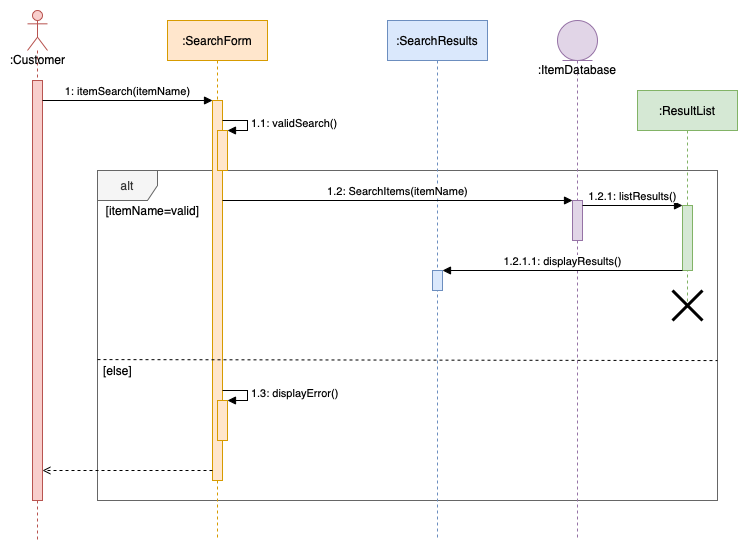
\includegraphics[width=0.8\textwidth]{figures/example_sequence_diagram.png}
    \caption{Beispiel für eine Aufrufhierarchie}
    \label{fig:example_sequence_diagram}
\end{figure}